\documentclass[11pt]{article}

\usepackage{amsmath,amssymb,mathtools}
\usepackage[margin=1in]{geometry}
\usepackage{enumitem}
\usepackage{xcolor}
\usepackage{microtype}
\usepackage{graphicx}
\usepackage{tikz,float}
\usepackage{subcaption}
\usepackage{amsthm}
\usepackage{hyperref}
\usepackage{array}
\usepackage{pgfplots}

\usetikzlibrary{shapes.geometric, arrows.meta, positioning, calc, decorations.markings}
\tikzset{
	block/.style={rectangle, draw, text width=6em, text centered, rounded corners, minimum height=10mm},
	sum/.style={circle, draw, node distance=1.5cm},
	line/.style={draw, -{Stealth[length=2.5mm, width=1.5mm]}}
}

\usepgfplotslibrary{groupplots}
\pgfplotsset{compat=1.18}

\pgfplotsset{
	myaxes/.style={
		axis lines=middle,
		axis line style={-latex},
		grid=major,
		grid style={gray!15},
		minor grid style={gray!35},
		xlabel style={at={(ticklabel* cs:1)}, anchor=north west},
		ylabel style={at={(ticklabel* cs:1)}, anchor=south east},
		every axis plot/.append style={thick}
	},
	myplotstyle/.style={
		width=14cm,
		height=7cm,
		axis lines=middle,
		axis line style={-Stealth},
		grid=both,
		minor tick num=1,
		major grid style={draw=gray!30},
		minor grid style={draw=gray!15},
		tick label style={font=\small, fill=white, inner sep=1.5pt},
		xlabel={$t$},
		ylabel={$x(t)$},
		xlabel style={anchor=north east, font=\small},
		ylabel style={anchor=south east, font=\small},
		samples=401,
	}
}

\newtheoremstyle{mynote}
{6pt}      % Space above
{6pt}      % Space below
{}          % Body font (normal, not italic)
{}          % Indent amount
{\bfseries} % Theorem head font
{.}         % Punctuation after theorem head
{.5em}      % Space after theorem head
{}          % Theorem head spec
\theoremstyle{mynote}
\newtheorem{definition}{Definition}
\newtheorem{proposition}{Proposition}
\newtheorem{example}{Example}
\newtheorem{remark}{Remark}
\newtheorem{theorem}{Theorem}
\newtheorem{corollary}{Corollary}

\newcommand{\T}{\mathcal{T}}
\newcommand{\R}{\mathbb{R}}
\newcommand{\Z}{\mathbb{Z}}
\newcommand{\C}{\mathbb{C}}
\newcommand{\conv}{\ast}
\newcommand{\dt}{\,\dd t}
\newcommand{\dd}{\mathrm{d}}
\newcommand{\imp}{\delta}
\newcommand{\sinc}[1]{\frac{\sin(\pi #1)}{\pi #1}}


\DeclareMathOperator{\rect}{rect}
\DeclareMathOperator{\Ev}{Ev}
\DeclareMathOperator{\Od}{Od}
\DeclareMathOperator{\sgn}{sgn}
\DeclareMathOperator{\step}{u}
\DeclareMathOperator{\tri}{tri}

\renewcommand{\qedsymbol}{}

\begin{document}
	% Reset figure counter for this lecture
	\renewcommand{\thefigure}{7.\arabic{figure}}
	
	% --- TITLE BLOCK ---
	\thispagestyle{empty}
	\noindent
	\begin{tabular*}{\textwidth}{l @{\extracolsep{\fill}} r}
		\textbf{Signals and Systems} & \textbf{Lecture 7} \\
		\textit{Dr. Ghandi Manasra and Ahmed Rabei} & \textit{Fall 2025} \\
	\end{tabular*}
	\hrule
	\vspace{0.4cm}
	\begin{center}
		\Large\textbf{Lecture 7: The Response of LTI Systems to Complex Exponentials \& Continuous-Time Fourier Series}
	\end{center}
	\vspace{0.4cm}
	
	\section*{Reference}
	Oppenheim \& Willsky, \textit{Signals and Systems}, Chapter 3, Sections 3.0--3.3
	
	\section*{Review of Lecture 6}
	\begin{itemize}[noitemsep]
		\item LTI properties from impulse response
		\item Causality and stability conditions
		\item LCCDEs in continuous and discrete time
		\item Implementation structures and realizations
	\end{itemize}
	
	\section*{7.1 Introduction}
	
	Last time, we connected the abstract properties of LTI systems to concrete conditions on their impulse responses. We established that:
	\begin{itemize}[noitemsep]
		\item \textbf{Causality} $\Leftrightarrow h(t)=0$ for $t<0$ (or $h[n]=0$ for $n<0$)
		\item \textbf{Stability} $\Leftrightarrow \int_{-\infty}^{\infty} |h(t)|\dd t < \infty$ (or $\sum_{n=-\infty}^{\infty} |h[n]| < \infty$)
	\end{itemize}
	
	We also introduced the most common way LTI systems are described in practice: linear constant-coefficient differential and difference equations. While convolution allows us to analyze these systems, the process can be cumbersome. Today, we begin to build a new, more powerful approach: frequency-domain analysis.
	
	The key insight is that complex exponentials have a special property when applied to LTI systems. This motivates us to represent signals as sums of complex exponentials. For periodic signals, we can use harmonically related complex exponentials, leading to the Fourier Series representation.
	\newpage
	\section*{7.2 Complex Exponentials as LTI Eigenfunctions}
	
	Let the input to a CT LTI system be $x(t) = e^{st}$ for any complex number $s$. The output is found by convolution:
	\[
	y(t) = \int_{-\infty}^{\infty} h(\tau) e^{s(t-\tau)}\dd\tau = e^{st} \int_{-\infty}^{\infty} h(\tau)e^{-s\tau}\dd\tau
	\]
	
	The integral is a complex constant $H(s)$ that depends on $s$ called \textbf{system function} $H(s)$:
	\[
	e^{st} \xrightarrow{\text{LTI System}} H(s)e^{st}
	\]
	
	For periodic complex exponentials, we set $s=j\omega$. The system function becomes the \textbf{frequency response}:
	\[
	H(j\omega) = \int_{-\infty}^{\infty} h(t)e^{-j\omega t}\dd t
	\]
	
	If the input is a sum of complex exponentials, by linearity:
	\[
	\text{If } x(t) = \sum_k a_k e^{j\omega_k t} \quad \implies \quad y(t) = \sum_k a_k H(j\omega_k) e^{j\omega_k t}
	\]
	
	This turns convolution into simple multiplication for each frequency component.
	
	\begin{figure}[H]
		\centering
		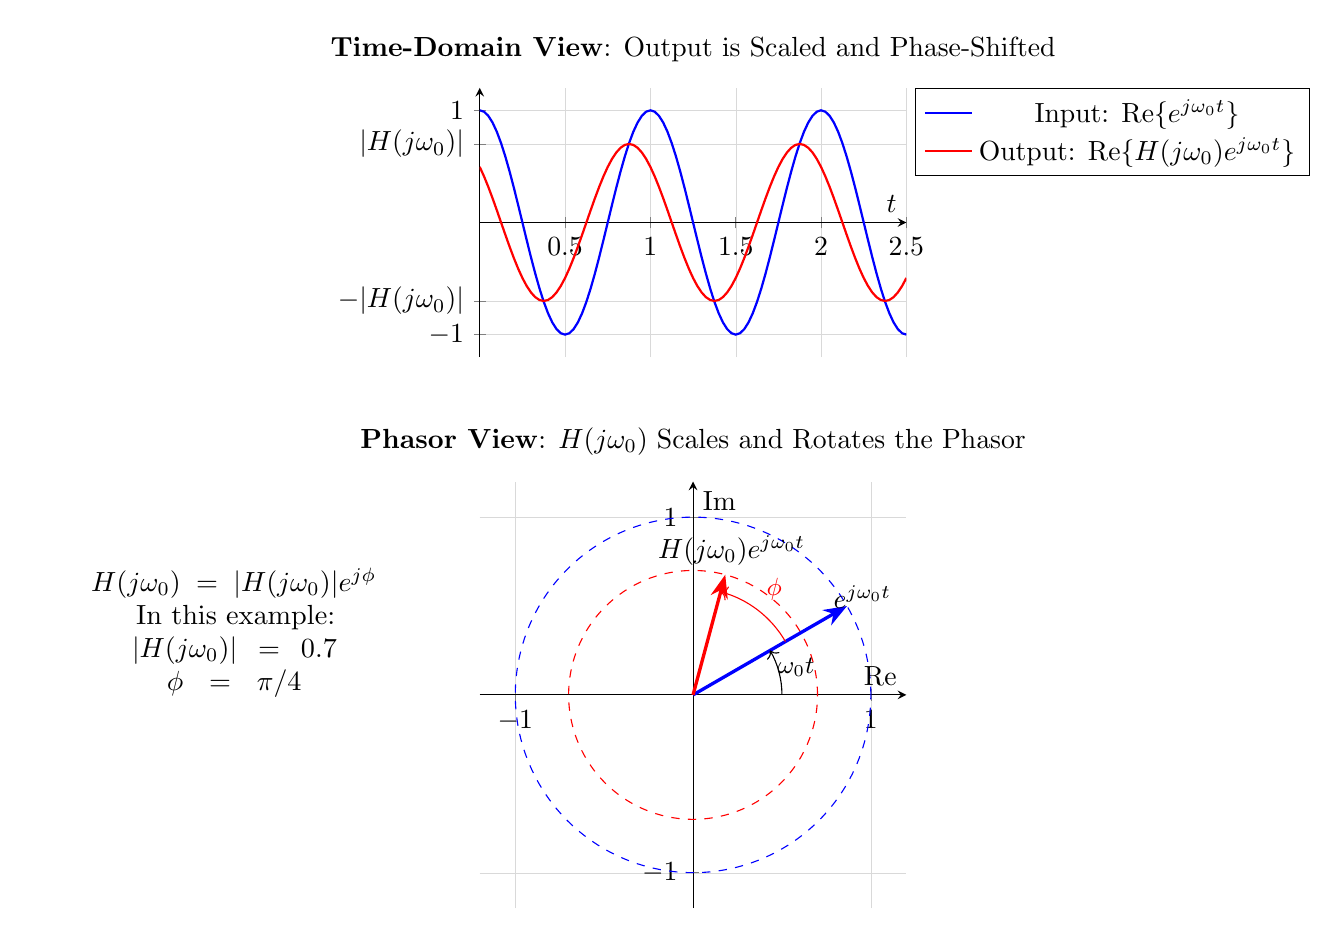
\begin{tikzpicture}
	
	%#####################################################################
	%### Top Plot: Time-Domain View (Amplitude Scaling & Phase Shift)
	%#####################################################################
	\begin{scope}[yshift=7cm]
		\begin{axis}[
			width=7cm, height=5cm,
			title={\textbf{Time-Domain View}: Output is Scaled and Phase-Shifted},
			xlabel={$t$},
			axis lines=middle,
			xmin=0, xmax=2.5, ymin=-1.2, ymax=1.2,
			xtick={0, 0.5, 1, 1.5, 2, 2.5},
			ytick={-1, -0.7, 0.7, 1},
			yticklabels={$-1$, $-|H(j\omega_0)|$, $|H(j\omega_0)|$, $1$},
			grid=major,
			grid style={line width=.1pt, draw=gray!30},
			legend style={at={(1.02,1)}, anchor=north west},
			no marks,
			]
			% Input Signal --- FIX: Increased samples for a smoother curve ---
			\addplot[blue, thick, domain=0:2.5, samples=101] {cos(deg(2*pi*x))};
			\addlegendentry{Input: $\text{Re}\{e^{j\omega_0 t}\}$};
			
			% Output Signal --- FIX: Increased samples for a smoother curve ---
			\addplot[red, thick, domain=0:2.5, samples=101] {0.7*cos(deg(2*pi*x) + 45)};
			\addlegendentry{Output: $\text{Re}\{H(j\omega_0)e^{j\omega_0 t}\}$};
			
		\end{axis}
	\end{scope}
	
	%#####################################################################
	%### Bottom Plot: Phasor View (Scaling & Rotation)
	%#####################################################################
	\begin{scope}[yshift=0cm]
		\begin{axis}[
			width=7cm, height=7cm,
			title={\textbf{Phasor View}: $H(j\omega_0)$ Scales and Rotates the Phasor},
			xlabel={$\text{Re}$}, ylabel={$\text{Im}$},
			axis equal image,
			axis lines=middle,
			xmin=-1.2, xmax=1.2, ymin=-1.2, ymax=1.2,
			xtick={-1, 1}, ytick={-1, 1},
			grid=major,
			grid style={line width=.1pt, draw=gray!30},
			]
			% Paths for input and output circles
			\addplot[blue, dashed, domain=0:360, samples=361, no marks] ({cos(x)}, {sin(x)});
			\addplot[red, dashed, domain=0:360, samples=361, no marks] ({0.7*cos(x)}, {0.7*sin(x)});
			
			% Define angle for a snapshot in time
			\pgfmathsetmacro{\wT}{30} % omega*t = 30 degrees
			
			% Coordinates
			\coordinate (O) at (axis cs:0,0);
			\coordinate (P_in) at (axis cs:{cos(\wT)}, {sin(\wT)});
			\coordinate (P_out) at (axis cs:{0.7*cos(\wT+45)}, {0.7*sin(\wT+45)});
			
			% Draw the phasors
			\draw[-{Stealth[blue]}, blue, very thick] (O) -- (P_in) node[pos=1.1, black] {$e^{j\omega_0 t}$};
			\draw[-{Stealth[red]}, red, very thick] (O) -- (P_out) node[pos=1.2, black] {$H(j\omega_0)e^{j\omega_0 t}$};
			
			% Angle omega*t
			\draw[->] (axis cs:0.5,0) arc[start angle=0, end angle=\wT, radius=0.5];
			\node at (axis cs:{0.6*cos(\wT/2)}, {0.6*sin(\wT/2)}) [font=\small] {$\omega_0 t$};
			
			% Angle phi
			\draw[->, red] (axis cs:{0.6*cos(\wT)}, {0.6*sin(\wT)}) arc[start angle=\wT, end angle={\wT+45}, radius=0.6];
			\node at (axis cs:{0.75*cos(\wT+22.5)}, {0.75*sin(\wT+22.5)}) [font=\small, red] {$\phi$};
			
		\end{axis}
	\end{scope}
	
	% Add an overall annotation
	\node[text width=5cm, align=center, anchor=east] at (-0.5, 3.5)
	 {$H(j\omega_0) = |H(j\omega_0)| e^{j\phi}$ \\ In this example: \\ $|H(j\omega_0)| = 0.7$ \\ $\phi = \pi/4$};
	
\end{tikzpicture}
		\caption{Complex exponentials pass through LTI systems with scaling only.}
		\label{fig:eigenfunction_property}
	\end{figure}
	
	
	\section*{7.3 The Continuous-Time Fourier Series (CTFS)}
	
	The insight from the previous section motivates us to represent periodic signals as a sum of harmonically related complex exponentials. This representation is the \textbf{Fourier Series}.
	
	\subsection*{7.3.1 Synthesis Equation}
	
	For a periodic signal $x(t)$ with fundamental period $T_0$ and frequency $\omega_0=2\pi/T_0$, its Fourier series representation is:
	\[
	x(t) = \sum_{k=-\infty}^{\infty} a_k e^{jk\omega_0 t}
	\]
	
	\begin{itemize}[noitemsep]
		\item The terms for $k=\pm 1$ are the \textbf{fundamental components}
		\item The terms for $k=\pm n$ are the \textbf{$n^{th}$ harmonics}
		\item The coefficients $a_k$ are the \textbf{Fourier series coefficients}, which encode information about both the magnitude and phase of each harmonic component in the signal
	\end{itemize}
	
	\subsection*{7.3.2 Analysis Equation}
	
	To find the coefficients, we can exploit the orthogonality of the harmonic components. The formula for the coefficients is:
	\[
	a_k = \frac{1}{T_0} \int_{T_0} x(t)e^{-jk\omega_0 t}\dd t
	\]
	
	The integral can be taken over \textit{any} interval of length $T_0$.
	
	\subsection*{7.3.3 Orthogonality Property}
	
	The harmonically related complex exponentials are orthogonal over a period:
	\[
	\int_{T_0} e^{jk\omega_0 t} e^{-jn\omega_0 t} \dd t = \begin{cases}
		T_0 & \text{if } k = n \\
		0 & \text{if } k \neq n
	\end{cases}
	\]
	
	\begin{proof}
		For $k \neq n$:
		\[
		\int_{T_0} e^{j(k-n)\omega_0 t} \dd t = \frac{1}{j(k-n)\omega_0} \left[ e^{j(k-n)\omega_0 t} \right]_{0}^{T_0} = \frac{1}{j(k-n)\omega_0} \left( e^{j(k-n)2\pi} - 1 \right) = 0
		\]
		since $e^{j(k-n)2\pi} = 1$ for integer $(k-n)$.
		
		For $k = n$:
		\[
		\int_{T_0} e^{j(k-n)\omega_0 t} \dd t = \int_{T_0} 1 \dd t = T_0
		\]
		\qed
	\end{proof}
	
	This orthogonality property enables precise extraction of each frequency component's contribution.
	
	\begin{figure}[H]
		\centering
		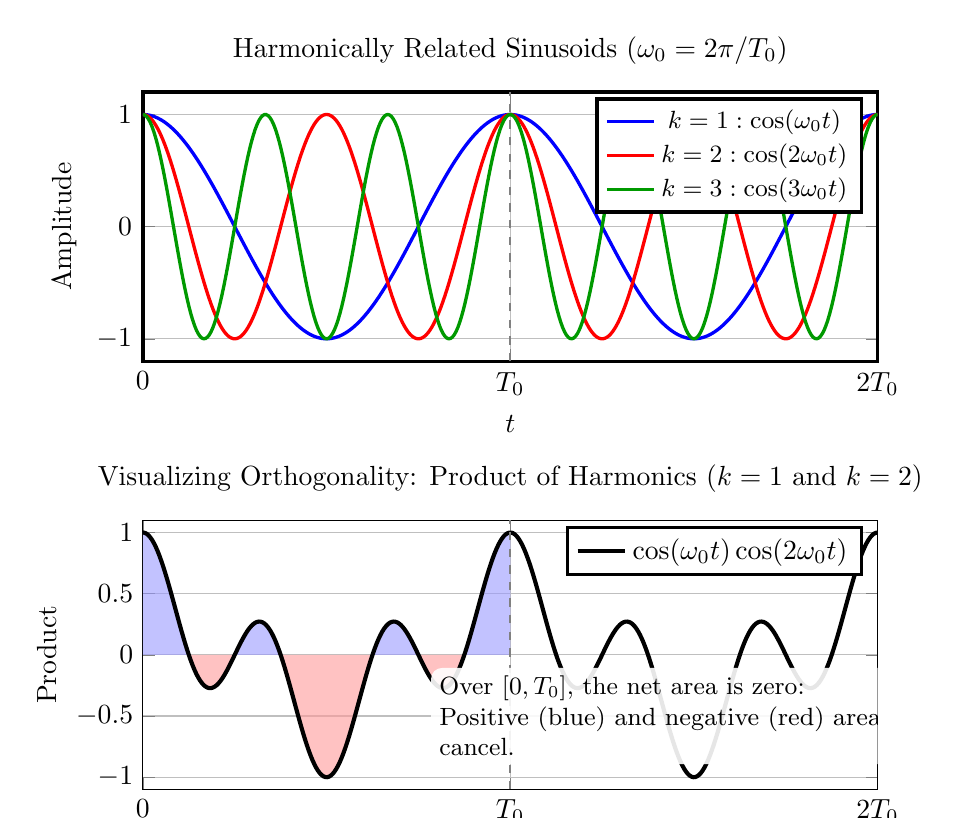
\begin{tikzpicture}
	\usepgfplotslibrary{fillbetween}
	
	% --- TOP PLOT: The Harmonics ---
	\begin{axis}[
		name=plot_harmonics,
		width=0.9\textwidth,
		height=5cm,
		title={Harmonically Related Sinusoids ($\omega_0 = 2\pi/T_0$)},
		xlabel={\(t\)},
		ylabel={Amplitude},
		grid=major,
		xmin=0, xmax=2,
		ymin=-1.2, ymax=1.2,
		xtick={0, 1, 2},
		xticklabels={\(0\), \(T_0\), \(2T_0\)},
		ytick={-1, 0, 1},
		legend style={at={(0.98,0.98)}, anchor=north east, font=\small},
		trig format plots=rad,
		samples=400,
		thick,
		no marks,
		line width=1.2pt,
		]
		% k=1 (Fundamental)
		\addplot[blue, domain=0:2] {cos(2*pi*x)};
		\addlegendentry{\(k=1: \cos(\omega_0 t)\)}
		
		% k=2
		\addplot[red, domain=0:2] {cos(4*pi*x)};
		\addlegendentry{\(k=2: \cos(2\omega_0 t)\)}
		
		% k=3
		\addplot[green!60!black, domain=0:2] {cos(6*pi*x)};
		\addlegendentry{\(k=3: \cos(3\omega_0 t)\)}
		
		% Period marker
		\draw[dashed, gray, thick] (axis cs:1,-1.2) -- (axis cs:1,1.2);
		\node[anchor=south, font=\footnotesize] at (axis cs:1,1.2) {\(T_0\)};
	\end{axis}
	
	% --- BOTTOM PLOT: Demonstrating Orthogonality ---
	\begin{axis}[
		at={(plot_harmonics.below south)},
		anchor=north,
		yshift=-1cm,
		width=0.9\textwidth,
		height=5cm,
		title={Visualizing Orthogonality: Product of Harmonics (\(k=1\) and \(k=2\))},
		xlabel={\(t\)},
		ylabel={Product},
		grid=major,
		xmin=0, xmax=2,
		ymin=-1.1, ymax=1.1,
		xtick={0, 1, 2},
		xticklabels={\(0\), \(T_0\), \(2T_0\)},
		ytick={-1, -0.5, 0, 0.5, 1},
		trig format plots=rad,
		samples=400,
		thick,
		no marks,
		line width=1.2pt,
		]
		% Plot the product of the first two harmonics
		\addplot[name path=product, domain=0:2, black, line width=1.5pt] 
		{cos(2*pi*x) * cos(4*pi*x)};
		\addlegendentry{\(\cos(\omega_0 t)\cos(2\omega_0 t)\)}
		
		% Path for the x-axis (to fill between)
		\path[name path=xaxis] (axis cs:0,0) -- (axis cs:2,0);
		
		% Fill the area between the product curve and x-axis over [0, T_0]
		\addplot[draw=none] fill between[
		of=product and xaxis,
		soft clip={domain=0:1},
		split,
		every even segment/.style={fill=blue!40, opacity=0.6},
		every odd segment/.style={fill=red!40, opacity=0.6},
		];
		
		% Period marker
		\draw[dashed, gray, thick] (axis cs:1,-1.1) -- (axis cs:1,1.1);
		\node[anchor=south, font=\footnotesize] at (axis cs:1,1.1) {\(T_0\)};
		
		% Annotation explaining the concept
		\node[align=left, text width=6cm, font=\small, fill=white, fill opacity=0.9, 
		text opacity=1, rounded corners, inner sep=3pt] at (axis cs:1.45, -0.5) {
			Over \([0, T_0]\), the net area is zero:\\
			Positive (blue) and negative (red) areas cancel.
		};
	\end{axis}
	
\end{tikzpicture}

		\caption{Harmonically related complex exponentials and their orthogonality.}
		\label{fig:orthogonality}
	\end{figure}
	
	\subsection*{7.3.4 Alternative Form: Trigonometric Fourier Series}
	
	While the complex exponential form is compact and mathematically convenient, the Fourier series can also be expressed as a sum of sines and cosines, which can be more intuitive for real signals.
	
	Any real periodic signal $x(t)$ can be written as:
	\[
	x(t) = A_0 + \sum_{k=1}^{\infty} \left( A_k \cos(k\omega_0 t) + B_k \sin(k\omega_0 t) \right)
	\]
	
	The coefficients are found by:
	\begin{align}
		A_0 &= \frac{1}{T_0} \int_{T_0} x(t) \dd t \\
		A_k &= \frac{2}{T_0} \int_{T_0} x(t) \cos(k\omega_0 t) \dd t \quad (k \geq 1) \\
		B_k &= \frac{2}{T_0} \int_{T_0} x(t) \sin(k\omega_0 t) \dd t \quad (k \geq 1)
	\end{align}
	\newpage
	\textbf{Relationship to Complex Coefficients:}
	The two forms are directly related. Given the complex coefficients $a_k$ for a real signal:
	\begin{itemize}[noitemsep]
		\item $A_0 = a_0$
		\item $A_k = 2 \text{Re}\{a_k\} = a_k + a_{-k}$
		\item $B_k = -2 \text{Im}\{a_k\} = j(a_k - a_{-k})$
	\end{itemize}
	
	Conversely, given the trigonometric coefficients:
	\begin{itemize}[noitemsep]
		\item $a_0 = A_0$
		\item $a_k = \frac{1}{2}(A_k - jB_k)$ for $k > 0$
		\item $a_{-k} = a_k^* = \frac{1}{2}(A_k + jB_k)$ for $k > 0$
	\end{itemize}
	
	
	\subsection*{7.3.5 Dirichlet Conditions for Convergence}
	
	The following are sufficient conditions for Fourier Series to converge:
	\begin{enumerate}[noitemsep]
		\item $x(t)$ must have at most a finite number of maxima and minima in one period
		\item $x(t)$ must have at most a finite number of discontinuities in one period
		\item $x(t)$ must be absolutely integrable over one period
	\end{enumerate}
	
\begin{theorem}[Convergence at Discontinuities]
	If $x(t)$ is a periodic function satisfying the Dirichlet conditions and $t_0$ is a point of jump discontinuity, then the Fourier Series converges pointwise to the midpoint value:
	\[
	\lim_{N \to \infty} \sum_{k=-N}^{N} a_k e^{jk\omega_0 t_0} = \frac{x(t_0^-) + x(t_0^+)}{2}
	\]
	where $x(t_0^-) = \lim_{t \to t_0^-} x(t)$ and $x(t_0^+) = \lim_{t \to t_0^+} x(t)$.
\end{theorem}

\begin{remark}
	For continuous signals, the Fourier Series converges uniformly to the original signal. For signals with discontinuities, convergence is pointwise except at discontinuities, where it converges to the midpoint value.
\end{remark}

	
	\section*{7.4 Examples}
	
	\subsection*{7.4.1 Fourier Coefficients for $x(t) = \sin(\omega_0 t)$}
	
	Using Euler's identity: $\sin(\omega_0 t) = \frac{1}{2j}e^{j\omega_0 t} - \frac{1}{2j}e^{-j\omega_0 t}$.
	
	By comparing this to the synthesis equation, we can see by inspection:
	\[
	a_1 = \frac{1}{2j}, \quad a_{-1} = -\frac{1}{2j}, \quad \text{and all other } a_k = 0
	\]
	
	\textbf{Explanation:} The sine wave contains just the fundamental frequency components at $+\omega_0$ and $-\omega_0$, with corresponding positive and negative phases.
	\newpage
	\subsection*{7.4.2 Fourier Series of a Periodic Square Wave}
	
	Let $x(t)$ be a square wave with period $T_0$ that equals 1 for $|t|<T_1$ and 0 for $T_1<|t|<T_0/2$.
	
	\begin{figure}[H]
		\centering
		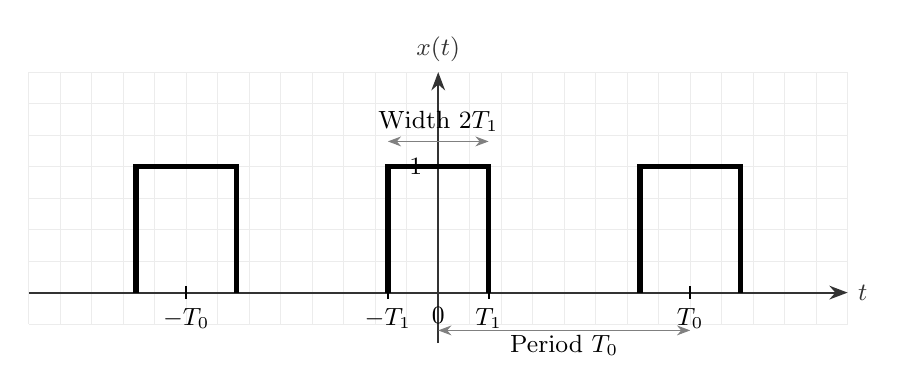
\begin{tikzpicture}[
	scale=0.8,
	>=Stealth,
	% --- Style Definitions ---
	axis/.style={->, thick, black!80},
	signal/.style={line width=2pt, blue!70!black},
	guideline/.style={dashed, gray!50, thin},
	dimline/.style={<->, thin, gray},
	annotation/.style={font=\small, inner sep=1.5pt},
	]
	
	% --- Parameters ---
	\def\A{2}           % Amplitude
	\def\Period{4}      % Period (T_0)
	\def\T1{0.8}        % Half pulse-width
	\def\Nperiods{1}    % Number of full periods to show left/right of the origin
	
	% --- Dynamic Boundaries ---
	\pgfmathsetmacro{\Xmax}{\Nperiods*\Period + \Period/2 + 0.5}
	\pgfmathsetmacro{\Xmin}{-\Xmax}
	\pgfmathsetmacro{\Ymax}{\A + 1.5}
	
	% --- Grid & Axes ---
	\draw[step=0.5, gray!15, very thin] (\Xmin,-0.5) grid (\Xmax,\Ymax);
	\draw[axis] (\Xmin, 0) -- (\Xmax, 0) node[right, font=\small] {$t$};
	\draw[axis] (0, -0.8) -- (0, \Ymax) node[above, font=\small] {$x(t)$};
	
	% --- Signal Drawing ---
	% Draw pulses (black for non-zero areas)
	\foreach \n in {-\Nperiods,...,\Nperiods} {
		\pgfmathsetmacro{\center}{\n*\Period}
		\draw[line width=2pt, black] (\center-\T1, 0) -- (\center-\T1, \A) -- (\center+\T1, \A) -- (\center+\T1, 0);
	}
	
	% --- Y-Axis Tick & Label ---
	\draw[thick] (-0.1, \A) -- (0.1, \A);
	\node[left, font=\small] at (-0.1, \A) {$1$};
	
	% --- X-Axis Ticks & Labels ---
	\node[below=2pt, font=\small] at (0,0) {$0$};
	% Only show T1 labels near origin
	\draw[thick] (-\T1, -0.1) -- (-\T1, 0.1);
	\node[below, font=\small] at (-\T1, -0.1) {$-T_1$};
	\draw[thick] (\T1, -0.1) -- (\T1, 0.1);
	\node[below, font=\small] at (\T1, -0.1) {$T_1$};
	% Show Period labels further out
	\draw[thick] (\Period, -0.1) -- (\Period, 0.1);
	\node[below, font=\small] at (\Period, -0.1) {$T_0$};
	\draw[thick] (-\Period, -0.1) -- (-\Period, 0.1);
	\node[below, font=\small] at (-\Period, -0.1) {$-T_0$};
	
	% --- Dimension Line for Period ---
	\draw[dimline] (0, -0.6) -- (\Period, -0.6);
	\node[below, annotation] at (\Period/2, -0.6) {Period $T_0$};
	
	% --- Dimension Line for Pulse Width ---
	\pgfmathsetmacro{\dimheight}{\A + 0.4}
	\draw[dimline] (-\T1, \dimheight) -- (\T1, \dimheight);
	\node[above=2pt, annotation] at (0, \dimheight) {Width $2T_1$};
	
\end{tikzpicture}

		\caption{Periodic rectangular pulse train with period $T_0$ and pulse width $2T_1$.}
		\label{fig:pulse_train}
	\end{figure}
	
	\begin{itemize}[noitemsep]
		\item The DC component ($k=0$) is the average value: $a_0 = \frac{1}{T_0}\int_{-T_1}^{T_1} 1 \dd t = \frac{2T_1}{T_0}$
		\item For $k \neq 0$:
		\[
		a_k = \frac{1}{T_0}\int_{-T_1}^{T_1} e^{-jk\omega_0 t}\dd t = \frac{2\sin(k\omega_0 T_1)}{k\omega_0 T_0} = \frac{\sin(k\omega_0 T_1)}{k\pi}
		\]
		This is a sinc-like function. For a symmetric square wave ($T_1 = T_0/4$), only odd harmonics appear with amplitude decaying as $1/k$.
	\end{itemize}
	
	\subsection*{7.4.3 Duty-Cycle Rectangular Pulse Train}
	
	For a rectangular pulse train with duty cycle $D = 2T_1/T_0$, we can generalize the square wave result. First, let us define the normalized sinc function:
	
	\begin{definition}[Normalized Sinc Function]
		The normalized sinc function is defined as:
		\[
		\text{sinc}(x) = \frac{\sin(\pi x)}{\pi x}
		\]
		with the special case $\text{sinc}(0) = 1$.
	\end{definition}
	
	Starting from our previous result for the centered pulse:
	\[
	a_k = \frac{\sin(k\omega_0 T_1)}{k\pi}
	\]
	
	Substituting $\omega_0 = 2\pi/T_0$ and $D = 2T_1/T_0$:
	\[
	a_k = \frac{\sin(k\pi (2T_1/T_0))}{k\pi} = \frac{\sin(k\pi D)}{k\pi}
	\]
	
	To express this in terms of the sinc function, we multiply and divide by $D$:
	\[
	a_k = D \cdot \frac{\sin(k\pi D)}{k\pi D} = D \cdot \text{sinc}(kD)
	\]
	\newpage
	\textbf{Key Points:}
	\begin{itemize}[noitemsep]
		\item Since the pulse is centered at $t=0$, the coefficients are real (no phase term)
		\item The magnitude follows the sinc envelope: $|a_k| = D|\text{sinc}(kD)|$
		\item For a square wave ($D = 1/2$), we get the familiar $1/k$ decay for odd harmonics
	\end{itemize}
	
	\begin{figure}[H]
		\centering
		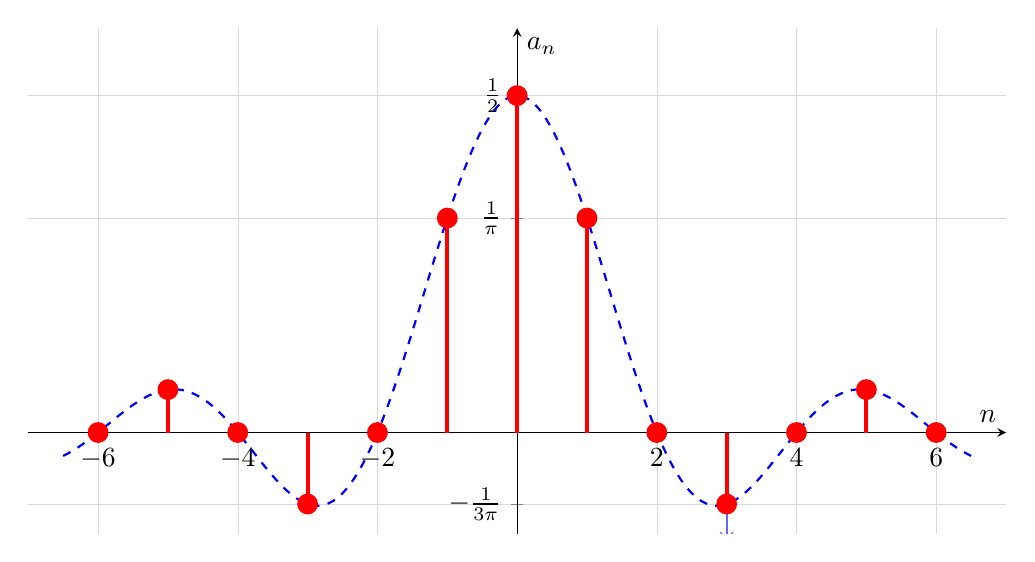
\begin{tikzpicture}
\begin{axis}[
    width=14cm,
    height=8cm,
    xlabel={$n$},
    ylabel={$a_n$},
    axis lines=middle,
    xmin=-7, xmax=7,
    ymin=-0.15, ymax=0.6,
    xtick={-6, -4, -2, 0, 2, 4, 6},
    ytick={-0.106103, 0, 0.318310, 0.5},
    yticklabels={$-\frac{1}{3\pi}$, $0$, $\frac{1}{\pi}$, $\frac{1}{2}$},
    grid=major,
    grid style={line width=.1pt, draw=gray!30},
    legend pos=north east,
]

% Plot the continuous sinc envelope
\addplot[
    blue,
    thick,
    dashed,
    domain=-6.5:6.5,
    samples=401,
] {0.5*(abs(x) < 0.01 ? 1 : sin(0.5*pi*deg(x))/(0.5*pi*x))};
% Plot the discrete samples as stems
\addplot+[
    red,
    ycomb,
    mark=*,
    mark options={fill=red, scale=1.5},
    thick,
    line width=1.5pt,
] table {
    x   y
   -6   0.000000
   -5   0.063662
   -4   0.000000
   -3   -0.106103
   -2   0.000000
   -1   0.318310
    0   0.500000
    1   0.318310
    2   0.000000
    3   -0.106103
    4   0.000000
    5   0.063662
    6   0.000000
};

% Annotations

\node[pin={[pin edge={-Stealth, thick, blue!60}]270:{Side Lobe}}] 
    at (axis cs:3,-0.106103) {};

\node[font=\small, fill=white, fill opacity=0.85, text opacity=1, 
      rounded corners, inner sep=3pt] 
    at (axis cs:0,-0.18)
    {Zeros at $t = \pm 2, \pm 4, \pm 6, \ldots$};

\end{axis}
\end{tikzpicture}
		\caption{Fourier series coefficients for a rectangular pulse train showing the sinc envelope and discrete samples of a square wave with duty cycle $50\%$}
		\label{fig:sinc_envelope}
	\end{figure}
	
	\begin{figure}[H]
		\centering
		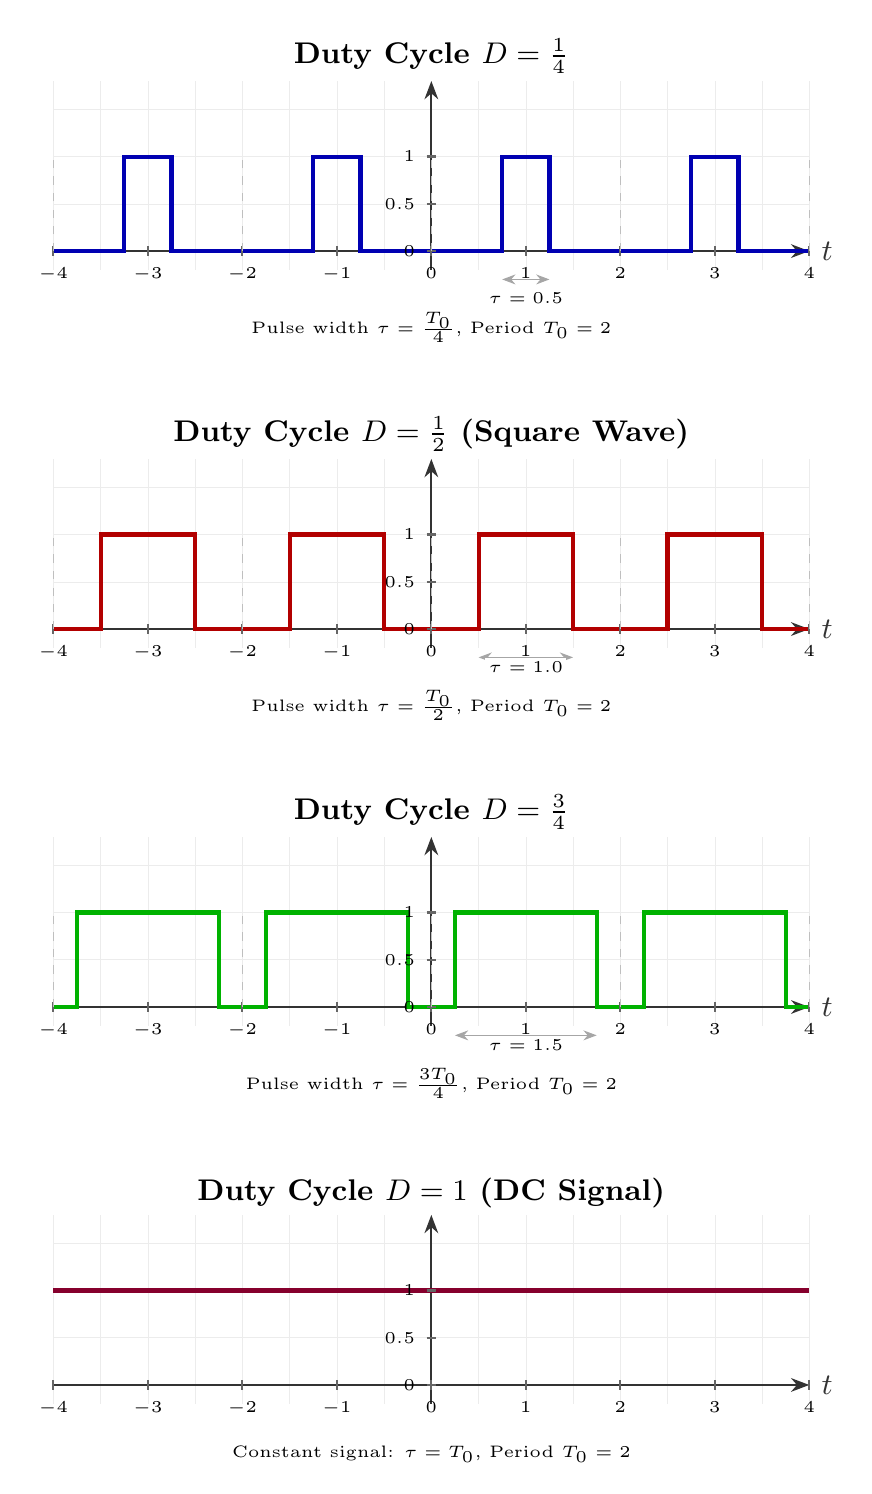
\begin{tikzpicture}[
	scale=1.2,
	>=Stealth,
	% --- Style Definitions ---
	transform shape,
	axis/.style={->, thick, black!80},
	signal/.style={line width=1.5pt},
	grid/.style={step=0.5, gray!15, very thin},
	tick/.style={thick, black!60},
	title/.style={font=\small\bfseries, fill=white, inner sep=2pt},
	annotation/.style={font=\tiny, fill=white, inner sep=1pt},
	dimline/.style={<->, thin, gray!70},
	]
	
	% --- Common Parameters ---
	\def\period{2}        % Period T_0
	\def\amplitude{1}     % Signal amplitude
	\def\xmin{-4}         % Show 2 periods on each side
	\def\xmax{4}
	\def\ymin{-0.2}
	\def\ymax{1.8}
	
	% --- Plot 1: D = 1/4 (Top) ---
	\begin{scope}[xshift=0cm, yshift=12cm]
		% Grid & Axes
		\draw[grid] (\xmin,\ymin) grid (\xmax,\ymax);
		\draw[axis] (\xmin, 0) -- (\xmax, 0) node[right, font=\small] {$t$};
		\draw[axis] (0, \ymin) -- (0, \ymax) node[above, font=\small] {$x(t)$};
		
		% Signal: D=1/4 means pulse width = 0.5, show multiple periods
		\draw[signal, blue!70!black] (\xmin, 0) -- (-3.25, 0) -- (-3.25, \amplitude) -- (-2.75, \amplitude) -- (-2.75, 0) -- (-1.25, 0) -- (-1.25, \amplitude) -- (-0.75, \amplitude) -- (-0.75, 0) -- (0.75, 0) -- (0.75, \amplitude) -- (1.25, \amplitude) -- (1.25, 0) -- (2.75, 0) -- (2.75, \amplitude) -- (3.25, \amplitude) -- (3.25, 0) -- (\xmax, 0);
		
		% Ticks and labels
		\foreach \x in {-4,-3,-2,-1,0,1,2,3,4} {
			\draw[tick] (\x, -0.05) -- (\x, 0.05);
			\node[below, font=\tiny] at (\x, -0.05) {$\x$};
		}
		\foreach \y in {0,0.5,1} {
			\draw[tick] (-0.05, \y) -- (0.05, \y);
			\node[left, font=\tiny] at (-0.05, \y) {$\y$};
		}
		
		% Period markers
		\draw[dashed, gray!50] (-4, 0) -- (-4, \amplitude);
		\draw[dashed, gray!50] (-2, 0) -- (-2, \amplitude);
		\draw[dashed, gray!50] (0, 0) -- (0, \amplitude);
		\draw[dashed, gray!50] (2, 0) -- (2, \amplitude);
		\draw[dashed, gray!50] (4, 0) -- (4, \amplitude);
		
		% Duty cycle annotation - positioned below the period from -1 to 1
		\draw[dimline] (0.75, -0.3) -- (1.25, -0.3);
		\node[below, annotation] at (1, -0.4) {$\tau = 0.5$};
		
		% Title
		\node[title, above] at (0, \ymax) {Duty Cycle $D = \frac{1}{4}$};
		\node[annotation, below] at (0, \ymin-0.4) {Pulse width $\tau = \frac{T_0}{4}$, Period $T_0 = 2$};
	\end{scope}
	
	% --- Plot 2: D = 1/2 (Second) ---
	\begin{scope}[xshift=0cm, yshift=8cm]
		% Grid & Axes
		\draw[grid] (\xmin,\ymin) grid (\xmax,\ymax);
		\draw[axis] (\xmin, 0) -- (\xmax, 0) node[right, font=\small] {$t$};
		\draw[axis] (0, \ymin) -- (0, \ymax) node[above, font=\small] {$x(t)$};
		
		% Signal: D=1/2 means pulse width = 1, show multiple periods
		\draw[signal, red!70!black] (\xmin, 0) -- (-3.5, 0) -- (-3.5, \amplitude) -- (-2.5, \amplitude) -- (-2.5, 0) -- (-1.5, 0) -- (-1.5, \amplitude) -- (-0.5, \amplitude) -- (-0.5, 0) -- (0.5, 0) -- (0.5, \amplitude) -- (1.5, \amplitude) -- (1.5, 0) -- (2.5, 0) -- (2.5, \amplitude) -- (3.5, \amplitude) -- (3.5, 0) -- (\xmax, 0);
		
		% Ticks and labels
		\foreach \x in {-4,-3,-2,-1,0,1,2,3,4} {
			\draw[tick] (\x, -0.05) -- (\x, 0.05);
			\node[below, font=\tiny] at (\x, -0.05) {$\x$};
		}
		\foreach \y in {0,0.5,1} {
			\draw[tick] (-0.05, \y) -- (0.05, \y);
			\node[left, font=\tiny] at (-0.05, \y) {$\y$};
		}
		
		% Period markers
		\draw[dashed, gray!50] (-4, 0) -- (-4, \amplitude);
		\draw[dashed, gray!50] (-2, 0) -- (-2, \amplitude);
		\draw[dashed, gray!50] (0, 0) -- (0, \amplitude);
		\draw[dashed, gray!50] (2, 0) -- (2, \amplitude);
		\draw[dashed, gray!50] (4, 0) -- (4, \amplitude);
		
		% Duty cycle annotation - positioned below the period from -1 to 1
		\draw[dimline] (0.5, -0.3) -- (1.5, -0.3);
		\node[below, annotation] at (1, -0.3) {$\tau = 1.0$};
		
		% Title
		\node[title, above] at (0, \ymax) {Duty Cycle $D = \frac{1}{2}$ (Square Wave)};
		\node[annotation, below] at (0, \ymin-0.4) {Pulse width $\tau = \frac{T_0}{2}$, Period $T_0 = 2$};
	\end{scope}
	
	% --- Plot 3: D = 3/4 (Third) ---
	\begin{scope}[xshift=0cm, yshift=4cm]
		% Grid & Axes
		\draw[grid] (\xmin,\ymin) grid (\xmax,\ymax);
		\draw[axis] (\xmin, 0) -- (\xmax, 0) node[right, font=\small] {$t$};
		\draw[axis] (0, \ymin) -- (0, \ymax) node[above, font=\small] {$x(t)$};
		
		% Signal: D=3/4 means pulse width = 1.5, show multiple periods
		\draw[signal, green!70!black] (\xmin, 0) -- (-3.75, 0) -- (-3.75, \amplitude) -- (-2.25, \amplitude) -- (-2.25, 0) -- (-1.75, 0) -- (-1.75, \amplitude) -- (-0.25, \amplitude) -- (-0.25, 0) -- (0.25, 0) -- (0.25, \amplitude) -- (1.75, \amplitude) -- (1.75, 0) -- (2.25, 0) -- (2.25, \amplitude) -- (3.75, \amplitude) -- (3.75, 0) -- (\xmax, 0);
		
		% Ticks and labels
		\foreach \x in {-4,-3,-2,-1,0,1,2,3,4} {
			\draw[tick] (\x, -0.05) -- (\x, 0.05);
			\node[below, font=\tiny] at (\x, -0.05) {$\x$};
		}
		\foreach \y in {0,0.5,1} {
			\draw[tick] (-0.05, \y) -- (0.05, \y);
			\node[left, font=\tiny] at (-0.05, \y) {$\y$};
		}
		
		% Period markers
		\draw[dashed, gray!50] (-4, 0) -- (-4, \amplitude);
		\draw[dashed, gray!50] (-2, 0) -- (-2, \amplitude);
		\draw[dashed, gray!50] (0, 0) -- (0, \amplitude);
		\draw[dashed, gray!50] (2, 0) -- (2, \amplitude);
		\draw[dashed, gray!50] (4, 0) -- (4, \amplitude);
		
		% Duty cycle annotation - positioned below the period from -1 to 1
		\draw[dimline] (0.25, -0.3) -- (1.75, -0.3);
		\node[below, annotation] at (1, -0.3) {$\tau = 1.5$};
		
		% Title
		\node[title, above] at (0, \ymax) {Duty Cycle $D = \frac{3}{4}$};
		\node[annotation, below] at (0, \ymin-0.4) {Pulse width $\tau = \frac{3T_0}{4}$, Period $T_0 = 2$};
	\end{scope}
	
	% --- Plot 4: D = 1 (Bottom) ---
	\begin{scope}[xshift=0cm, yshift=0cm]
		% Grid & Axes
		\draw[grid] (\xmin,\ymin) grid (\xmax,\ymax);
		\draw[axis] (\xmin, 0) -- (\xmax, 0) node[right, font=\small] {$t$};
		\draw[axis] (0, \ymin) -- (0, \ymax) node[above, font=\small] {$x(t)$};
		
		% Signal: D=1 means constant signal (DC)
		\draw[signal, purple!70!black] (\xmin, \amplitude) -- (\xmax, \amplitude);
		
		% Ticks and labels
		\foreach \x in {-4,-3,-2,-1,0,1,2,3,4} {
			\draw[tick] (\x, -0.05) -- (\x, 0.05);
			\node[below, font=\tiny] at (\x, -0.05) {$\x$};
		}
		\foreach \y in {0,0.5,1} {
			\draw[tick] (-0.05, \y) -- (0.05, \y);
			\node[left, font=\tiny] at (-0.05, \y) {$\y$};
		}
		
		% Title
		\node[title, above] at (0, \ymax) {Duty Cycle $D = 1$ (DC Signal)};
		\node[annotation, below] at (0, \ymin-0.4) {Constant signal: $\tau = T_0$, Period $T_0 = 2$};
	\end{scope}
	
\end{tikzpicture}
		\caption{Rectangular pulse trains with different duty cycles $D$.}
		\label{fig:duty_cycle_examples}
	\end{figure}
	
	\subsection*{7.4.4 Fourier Synthesis Demonstration}
	
	\begin{figure}[H]
		\centering
		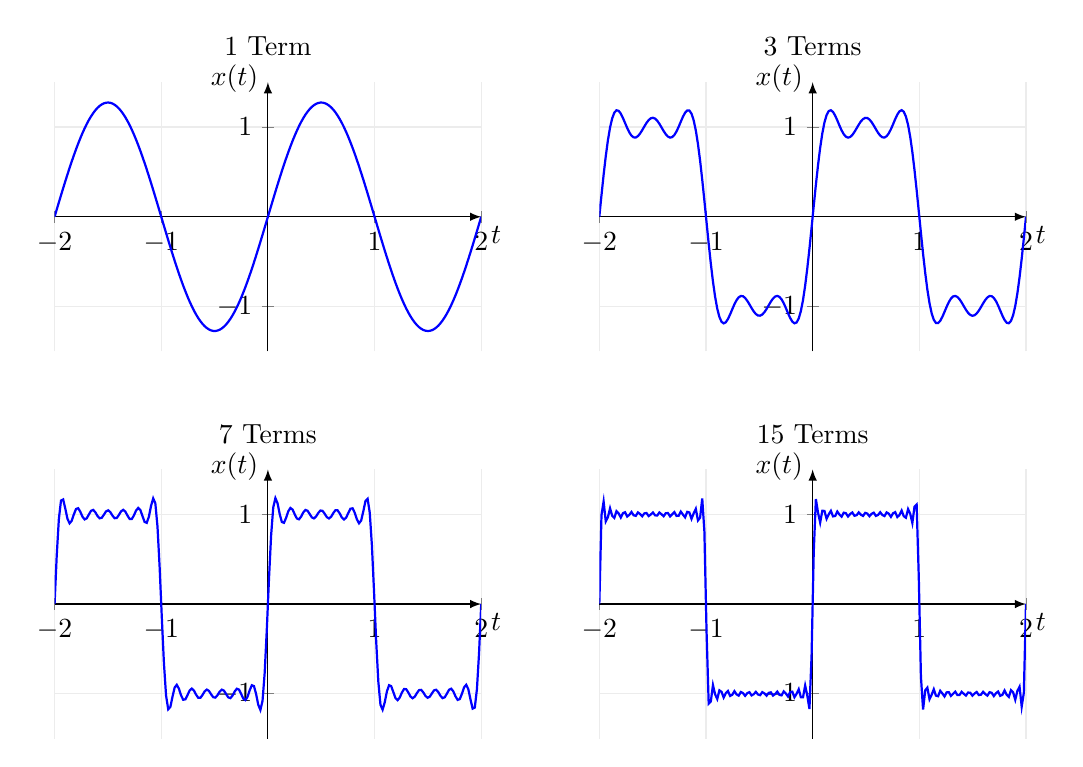
\begin{tikzpicture}
	\begin{groupplot}[
		group style={group size=2 by 2, horizontal sep=1.5cm, vertical sep=1.5cm},
		height=5cm, width=7cm,
		xlabel={$t$}, ylabel={$x(t)$},
		xmin=-2, xmax=2, ymin=-1.5, ymax=1.5,
		xtick={-2,-1,0,1,2},
		ytick={-1,0,1},
		axis lines=middle,
		axis line style={-latex},
		grid=major,
		grid style={gray!15},
		minor grid style={gray!35},
		xlabel style={at={(ticklabel* cs:1)}, anchor=north west},
		ylabel style={at={(ticklabel* cs:1.1)}, anchor=north east},
		every axis plot/.append style={thick}
	]
	\nextgroupplot[title={1 Term}]
	\addplot[blue, thick, domain=-2:2, samples=200] {4/pi * sin(deg(pi*x))};
	
	\nextgroupplot[title={3 Terms}]
	\addplot[blue, thick, domain=-2:2, samples=200] {4/pi * (sin(deg(pi*x)) + 1/3*sin(deg(3*pi*x)) + 1/5*sin(deg(5*pi*x)))};
	
	\nextgroupplot[title={7 Terms}]
	\addplot[blue, thick, domain=-2:2, samples=200] {4/pi * (sin(deg(pi*x)) + 1/3*sin(deg(3*pi*x)) + 1/5*sin(deg(5*pi*x)) + 1/7*sin(deg(7*pi*x)) + 1/9*sin(deg(9*pi*x)) + 1/11*sin(deg(11*pi*x)) + 1/13*sin(deg(13*pi*x)))};
	
	\nextgroupplot[title={15 Terms}]
	\addplot[blue, thick, domain=-2:2, samples=200] {4/pi * (sin(deg(pi*x)) + 1/3*sin(deg(3*pi*x)) + 1/5*sin(deg(5*pi*x)) + 1/7*sin(deg(7*pi*x)) + 1/9*sin(deg(9*pi*x)) + 1/11*sin(deg(11*pi*x)) + 1/13*sin(deg(13*pi*x)) + 1/15*sin(deg(15*pi*x)) + 1/17*sin(deg(17*pi*x)) + 1/19*sin(deg(19*pi*x)) + 1/21*sin(deg(21*pi*x)) + 1/23*sin(deg(23*pi*x)) + 1/25*sin(deg(25*pi*x)) + 1/27*sin(deg(27*pi*x)) + 1/29*sin(deg(29*pi*x)))};
	\end{groupplot}
\end{tikzpicture}

		\caption{Fourier synthesis showing convergence to square wave.}
		\label{fig:fourier_synthesis}
	\end{figure}
	
	
	\textbf{Key Observation:} Notice how the Gibbs phenomenon (overshoot) remains at ~9\% but gets squeezed to the discontinuity edges as more terms are added.
	
	
	
	\section*{7.5 Summary and Next Lecture}
	
	Today marks a fundamental shift in our approach. We have shown that complex exponentials are eigenfunctions of LTI systems, which means that analyzing systems in terms of these signals is algebraically simple.
	
	This motivated us to introduce the \textbf{Continuous-Time Fourier Series}, a tool for representing any periodic signal as a weighted sum of harmonically related complex exponentials. We now have a "recipe" for signals, where the ingredients are simple sinusoids.
	
	\textbf{Key Takeaways:}
	\begin{itemize}[noitemsep]
		\item Complex exponentials are LTI eigenfunctions: they pass through LTI systems unchanged except for scaling
		\item Fourier series lets us express any periodic signal as a sum of exponentials, with coefficients encoding amplitude and phase at each harmonic
		\item Time-domain convolution and differential equations correspond to simple multiplication or scaling in the frequency domain
	\end{itemize}
	
	\textbf{Next lecture:} We will explore the properties of the Fourier Series. We'll see how operations in the time domain, like shifting or differentiation, have simple and predictable effects on the Fourier series coefficients, further simplifying our analysis.
	
	By mastering these tools, signal analysis becomes more intuitive, algebraic, and powerful
	
\end{document}
